%! Author = petter
%! Date = 04.01.2021

\chapter{Implementation}\label{ch:implementation}

In this chapter we are going to look at the implementation for our compiler for PTS, as described in chapter~\vref{ch:the-language---pts}.
Before looking at the implementation we will first be discussing the methodology used during development.

\section{Methodology}\label{sec:methodology}

When tackling a project of this magnitude it is important to have a proper methodology for development.
During the development phase of this project I have had a strong focus on using agile techniques, where I have filled the role as both product owner and developer.
This agile software development has aided me in discovering new requirements as the project moves forward, and re-adjusting to these new requirements.
I have actively used a Kanban board throughout development to help keep track of tasks and goals.

The compiler was made in an iterative manner.
For each iteration I would start off by implementing a new feature, and then put on the product owner hat and test out the compiler.
While working as product owner I try to understand how I would like to use the language and what requirements I have for the language.
This often leads to re-adjusting the requirements.

I started off by creating a rough MVP (Minimum Viable Product), only implementing the most basic functionality, which comprised declaration of packages/templates and simple instantiation.
This MVP made me understand the project and requirements better, and also gave the project some new requirements.
After the initial iteration I decided to adopt a test-driven development approach.
I made tests for the features I had already implemented and then continued to make tests for the next functionality goal.
This was done in order to gain more confidence in the compiler, as well as helping me spot any erroneous code earlier rather than later, which makes fixing it less costly.
All of this resulted in a better development cycle, making refactoring and implementation of new features a breeze.
When adding new features or refactoring some tests will undoubtedly fail, and before moving on I made sure that all the tests were passing again.


\section{Compiler Architecture}\label{sec:architecture}

Our compiler consists of the following parts:

\begin{itemize}
    \item Lexing and parsing
    \item Parse tree transformation
    \item Type checking packages/templates
    \item Code generation
\end{itemize}

An overview of our architecture can be seen in figure~\vref{fig:compiler-overview}.
The first part of the compiler, namely the lexing and parsing will take a source file and transform it into a parse tree.
Our compiler will then take this parse tree and transform it into a simpler AST\@.
This simple AST will then be used to perform the PT transformations.
We will then use this AST to close any open packages and templates, and finally use the transformed tree for code generation.
After all packages and templates have been closed we can type-check each individual package/template to validate the type-safety of our program.
Given a valid type-safe program we can then move on to code generation.
The target language for our code generation will mainly be TypeScript, however we will also offer to transpile the TypeScript into JavaScript.

\begin{figure}
   \centering
   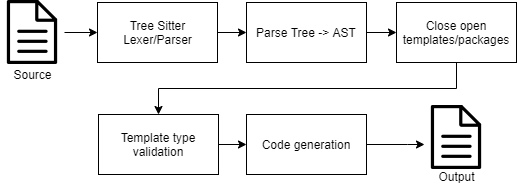
\includegraphics[scale=.75]{images/Compiler overview.png}
   \caption{Overview of the compiler}
   \label{fig:compiler-overview}
\end{figure}

\section{Lexer and Parser}\label{sec:lexer-and-parser}


\subsection{Parser Generator}\label{subsec:parser-generator}

There are a lot of parser generators out there, but there is no one-size-fits-all solution.
In order to navigate through the sea of options we need to set some requirements in functionality, so that we can more easily find the right tool for the task.

As we talked about in section~\vref{sec:what-do-we-need}, we set ourselves the goal to find an approach that would allow us to create an implementation that was loosely coupled with TypeScript.
TypeScript is a large language that is constantly updated, and is getting new features fairly often.
Because of this one of the requirements for our choice of parser generator is the possibility for extending grammars.
This is important because we want to keep our grammar loosely coupled with the TypeScript grammar, and don't want to be forced to rewrite the entire TypeScript grammar, as well as keeping it up-to-date.

We will be working with the TypeScript API, which only has a runtime library in JavaScript/TypeScript.
Therefore, another desired attribute is a runtime library in TypeScript.
This is not as essential as the requirement above, as we can get around using the TypeScript API and instead use the TypeScript CLI, or create a CLI in the language of the parser generator tools runtime library.


\subsubsection{ANTLR4}\label{subsubsec:antlr}

ANTLR, ANother Tool for Language Recognition, is a very powerful and versatile tool, used by many, such as Twitter for query parsing in their search engine\cite{Terence2012}.

ANTLR supports extending grammars, or more specifically importing them.
Importing a grammar works much like a "smart include".
It will include all rules that are not already defined in the grammar.
Through this you can extend a grammar with new rules or replacing them.
It does not however support extending rules, as in referencing the imported rule while overriding\cite{Terence2012}.
This isn't a major issue however as you could easily rewrite the rule with the additions.

The only supported runtime library in ANTLR is in Java.
This does not mean that you won't be able to use it in any other language, as you could simply invoke the runtime library through command line, however it is worth keeping in mind.

Overall ANTLR seems like a good option for our project, but the lack of a runtime library in TypeScript is a hurdle we would rather get a round if we can.

\subsubsection{Bison}\label{subsubsec:bison}

Bison is a general-purpose parser generator.
It is one of many successors to Yacc, and is upwards compatible with Yacc\cite{bison}.

Bison does not support extending grammars.
The tool works on a single grammar file and produces a C/C++ program.
There is a possibility to include files, like with any other C/C++ program, in the grammar files prologue, however this will not allow us to include another grammar, as it only inserts the prologue into the generated parser.
In order to extend a grammar we would have to change the produced parser to include some extra rules.
Although this could possibly be automated by a script, it seems too hacky of a solution to consider.

On top of this Bison does not have a runtime library in JavaScript/TypeScript.
There does exist some ports/clones of Bison for JavaScript, such as \href{http://zaa.ch/jison/}{Jison} and \href{http://canna71.github.io/Jacob/}{Jacob}, however to my knowledge these also lack the functionality of extending grammars.

\subsubsection{Tree-sitter}\label{subsubsec:tree-sitter}

\href{https://tree-sitter.github.io/tree-sitter/}{Tree-sitter} is a fairly new parser generator tool, compared to the others in this list.
It aims to be general, fast, robust and dependency-free\cite{tree-sitter}.
The tool has been garnering a lot of traction the last couple of years, and is being used by Github, VS Code and Atom to name a few.
It has mainly been used in language servers and syntax highlighting, however it should still work fine for our compiler since it does produce a parse tree.

Although it isn't a documented feature, Tree-sitter does allow for extending grammars.
Extending a grammar works much like in ANTLR, where you get almost a superclass relation to the grammar.
One difference from ANTLR though is that it does allow for referencing the grammar we are extending during rule overriding.
This makes it easier and more robust to extend rules than in ANTLR.

Tree-sitter also has a runtime library for TypeScript, which makes it easier for us to use it in our implementation than the previous candidates.

Another cherry on top is that Tree-sitter is becoming one of the mainstream ways of syntax highlighting in modern editors and IDEs, which means that we could utilize the same grammar to get syntax highlighting for our language.

All this makes Tree-sitter stand out as the best candidate for our project.

\subsubsection{Implementing Our Grammar in Tree-sitter}

Tree-sitter uses the term rule instead of production, and I will therefore also refer to productions as rules here.

Extending a grammar in Tree-sitter works much like extending a class in an object-oriented language.
A "sub grammar" inherits all the rules from the "super grammar", so an empty ruleset would effectively work the same as the super grammar.
Just like most object-oriented languages have access to the super class, we also have access to the super grammar in Tree-sitter.
All of this enables us to add, override, and extend rules in an existing grammar, all while staying loosely coupled with the super grammar.
By extending the grammar, and not forking it, we are able to simply update our dependency on the TypeScript grammar, minimizing the possibility for conflicts.

As mentioned, Tree-sitter allows for referencing the super grammar during rule overriding, effectively making it possible to combine the old rule and the new.
A good example of overriding and combining rules can be found in the grammar of PTS, see listing~\vref{lst:overriding-combining-rule}, where we override the \codeword{\_declaration} rule from the TypeScript grammar, to include the possibility for package and template declarations.

\begin{code}{javascript}{Snippet from the PTS grammar, where we override the \codeword{\_declaration} rule from the TypeScript grammar, and adding two additional declarations.}{lst:overriding-combining-rule}
    _declaration: ($, previous) =>
        choice(
            previous,
            $.template_declaration,
            $.package_declaration
        )
\end{code}




\section{Transforming Parse Tree to AST}\label{sec:transforming-parse-tree-to-ast}
%! Author = Petter
%! Date = 2/26/2021

\subsection{The AST Nodes}\label{subsec:the-ast-nodes}

Tree-sitter is a parser-generator written in Rust.
Fortunately for us we can still use tree-sitter in Node, due to Node supporting native addons\footnote{Node native addons are dynamically-linked shared objects written in C++\cite{nodenativeaddons}.}.
Native addons in Node are fairly new, and at the time of writing the tree-sitter Node bindings are still using the older unstable \hyperref[https://github.com/nodejs/nan]{NAN} instead of the newer and more stable \hyperref[https://nodejs.org/api/n-api.html]{napi}.
For the most part it does work, however I did meet some difficulties with the produced parse tree, more specifically the spread operator was not behaving properly on the native produced objects.
To get around this we will be walking through the parse tree and produce an AST.
What this means in practice is that we are going to be ignoring some parsing specific properties.
One of the changes we are going to make is that we are going to ignore if a node is named or unnamed, we will be keeping all nodes.
This will help us later in code generation.

For each AST node we picked out the following properties from the parse tree:

\begin{itemize}
    \item Node type
    \item Text
    \item Children
\end{itemize}

The node type is a string representing the rule which produced the node.
An AST node with a node type value of \codeword{"class\_declaration"} for instance is a class declaration node.

The text field of an AST node contains the textual representation/code for the node and its children.
A class declaration node for instance would of course contain the class declaration("\codeword{class A extend B \{}"), but also the entire body of the class.
This text field is really only useful for leaf nodes, as this would for instance contain the value of a number, string, etc.

Finally, the children field is, as the name would suggest, a list of all the children of the node.
For a class declaration node this would contain a leaf node containing the keyword \codeword{class}, a type identifier for the class name, and the class body.
Optionally it could also contain a class heritage node, which again contains either an extends clause, an implements clause or both.

We could have also opted to get the start position and end position of each node, so that we could use this to produce better error messages.
This was however not a priority in this thesis.

\subsection{Transforming}\label{subsec:transforming}

I chose to do the transforming immutable, and in order to do this we have to traverse the parse tree depth first and create nodes postfix.
Tree-sitter provides pretty nice functionality for traversing the parse tree through cursors.
With a tree cursor we are able to go to the parent, siblings, and children easily.
Using this we visit each node and produce an AST node as described in the section above.

\section{Closing Templates}\label{sec:closing-templates}
A closed template is a template that comprises only class, interface or enum declarations.
An open template on the other hand is a template that contains at least one instantiation statement.

The task of closing open packages and templates is what most of the implementation is focused around.
It is the task of performing the instantiations declared in the body of a package/template.

For instantiations without renaming the task is fairly simple.
We merely have to find the referenced template, and replace the instantiation statement with the body of said template.
Renaming on the other hand requires a bit more work.

In order to perform renaming on an instantiation we will have to perform the following tasks.
\begin{enumerate}
    \item Create a scope for the template body, and give all nodes of the body access to this scope
    \item Find all identifiers, member expressions, class declarations, etc., and replace them with \textit{reference nodes}\footnote{Reference nodes are AST nodes that contain a pointer to the class or field they are supposed to represent. This makes the task of renaming easier as we only have to worry about changing the name in one place. We will go into more detail about this in section~\vref{subsec:transforming-nodes-to-references}.}
    \item Perform the rename.
    \item Transform the scoped AST with reference nodes back to the original AST\@.
\end{enumerate}

If the template body is also open we would have to close it as well.
We want to close the nested templates before closing the upper templates, as renaming at the top level should affect all members from the nested instantiations.

Finally, once all templates have been closed we will have to perform class merging and apply any additions to classes.

In order to get a better understanding of this we will go through each step of closing a template in more detail.

%\begin{code}{}{Pseudocode for closing a template. The same code could also be used to close a package, as they are essentially equal in this regard.}{lst:pseudo-close-pacakge}
%    templates <- map from template name to body
%    FUNCTION close_template(template_body)
%        new_program <-
%            MAP syntax_node IN template_body
%                IF syntax_node IS instantiation statement THEN
%                    instantiated_template_body <- LOOKUP referenced template from instantiation statement IN templates
%                    closed_template_body <- close_template(instantiated_template_body)
%                    scoped_body <- add_scope(closed_template_body)
%
%                    renamings <- get renamings from instantiation statement
%                    FOR renaming IN
%                ELSE
%                    syntax_node
%                END IF
%            END MAP
%        RETURN new_program
%    END FUNCTION
%
%    FUNCTION
%\end{code}

\subsection{Scoping}\label{subsec:inst-scoping}

This step of closing templates works on the body of a copy of the instantiated template.
In order to be able to rename classes and class fields we first need to create correct scopes in which the renaming can be applied to.
We start of with a list of normal AST nodes and will transform these nodes into nodes that has a reference to the scope they are part of.

Scopes in the compiler mainly consists of three different classes.
The \codeword{Scope}, \codeword{Variable}, and \codeword{Class} classes.

The \codeword{Scope} class is essentially a symbol table that optionally extends a parent scope.
A scope without a reference to a parent scope is the root scope.
The symbol table is implemented as a map from the original field or class name, to a reference to either \codeword{Variable} or \codeword{Class} instance.
Looking up symbols in the symbol table will always start in the called scope, and work its way upwards until we reach the root scope.
This allows us to correctly handle shadowed variables.

The \codeword{Variable} class is a representation for class fields.
The class contains the name of the field.


For creating scopes I chose the following node types for "making new scopes".

\begin{multicols}{2}
\begin{itemize}
    \item \codeword{class\_body}
    \item \codeword{statement\_block}
    \item \codeword{enum\_body}
    \item \codeword{if\_statement}
    \item \codeword{else\_statement}
    \item \codeword{for\_statement}
    \item \codeword{for\_in\_statement}
    \item \codeword{while\_statement}
    \item \codeword{do\_statement}
    \item \codeword{try\_statement}
    \item \codeword{with\_statement}
\end{itemize}
\end{multicols}

\subsection{Transforming Nodes to References}\label{subsec:transforming-nodes-to-references}

Transforming nodes into references mainly consists of two steps.

\begin{itemize}
    \item Transform declarations
    \item Transform references
\end{itemize}

\subsubsection{Transform Declarations}

The task of transforming declarations requires several passes through the AST\@.
This is because in order to register som declarations we need to have others registered.
To understand this we can look at the difference between the first and second pass.

During the first pass through the AST we register and transform all class declarations.
Now for the second pass we register class heritage.
The second pass needs to update the \codeword{Class} instances from the first pass with what class they are extending.
If we try to do this in a single pass we would have to register classes

\subsubsection{Transform References}

\subsection{Performing the Rename}\label{subsec:performing-the-rename}

With all declarations and references transformed into reference nodes we can now perform the rename.
For each class rename we can simply lookup the old class name in the root scope and change the reference to the new class name.
For class field renames we do the same just for the enclosing classes scope.

\subsection{Going back to the original AST}\label{subsec:going-back-to-the-original-ast}


\section{Verification of Templates}\label{sec:verification-of-templates}

ts api

\section{Code Generation}\label{sec:code-generation}

After performing these steps we can finally produce the output.
Producing TypeScript output is a pretty simple task.
By traversing the AST we can concatenate the text from each leaf node and insert some whitespace between them.
This will produce quite ugly, unformatted code, but as long as the closed packages and templates are valid typescript programs this will also produce a valid typescript program.
In order to make it a bit more clean we perform an extra step before writing the output to the specified file, a formatting step.
There are a lot of TypeScript formatters out there, but we will be using \textit{Prettier} for our implementation.
Running our produced source code through the prettier formatter produces a nicely formatted, readable output.

Since browsers only support JavaScript we will also be implementing this as a target for code generation.
This is fortunately also a simple task, as we already dependent on the TypeScript compiler, and we are able to produce TypeScript source code, we can use this to produce JavaScript output.
% TODO: Undersøk  hvilken ES versjon vi outputter til og om dette kan være lavere.

\section{Notes on Performance}\label{sec:notes-on-performance}

Very slow compiler/PP because of the chosen implementation, with tree traverser for every step.


\section{Testing}\label{sec:testing}

Testing has been an essential part throughout the development of the compiler.
After the initial prototype of the compiler was running I continued onward with test driven development.
This allows me to write up tests for all the features of the language, and run them concurrently as I make the changes to the implementation.

The cycle

\subsection{Lexer and Parser}\label{subsec:testing-lexer-and-parser}

Tree-sitter tests are simple \codeword{.txt} files split up into three sections, the name of the test, the code that should be parsed, and the expected parse tree in \textit{S-expressions}\footnote{S-expressions are textual representations for tree-structured data. See~\cite{sexprs} for additional information and examples}.

\begin{code}{typescript}{Example of tree-sitter grammar test}{lst:tree-sitter-grammar-test}
    ===========================
    Closed template declaration
    ===========================

    template T {
        class A {
            i = 0;
        }
    }

    ---
    (program
        (template_declaration
            name: (identifier)
            body: (package_template_body
                    (class_declaration
                        name: (type_identifier)
                        body: (class_body
                            (public_field_definition
                                name: (property_identifier)
                                value: (number)))))))

\end{code}

\subsection{Transpiler}\label{subsec:testing-transpiler}

Started with jest, and used some time to get it to work with typescript files, however had to switch because jest doesn't handle native libraries (tree-sitter) too well.
It \codeword{require}s the same native library several times, making the wrapping around the native program to break.